
%% bare_conf_compsoc.tex
%% V1.4b
%% 2015/08/26
%% by Michael Shell
%% See:
%% http://www.michaelshell.org/
%% for current contact information.
%%
%% This is a skeleton file demonstrating the use of IEEEtran.cls
%% (requires IEEEtran.cls version 1.8b or later) with an IEEE Computer
%% Society conference paper.
%%
%% Support sites:
%% http://www.michaelshell.org/tex/ieeetran/
%% http://www.ctan.org/pkg/ieeetran
%% and
%% http://www.ieee.org/

%%*************************************************************************
%% Legal Notice:
%% This code is offered as-is without any warranty either expressed or
%% implied; without even the implied warranty of MERCHANTABILITY or
%% FITNESS FOR A PARTICULAR PURPOSE! 
%% User assumes all risk.
%% In no event shall the IEEE or any contributor to this code be liable for
%% any damages or losses, including, but not limited to, incidental,
%% consequential, or any other damages, resulting from the use or misuse
%% of any information contained here.
%%
%% All comments are the opinions http://www.bibtex.org/Using/of their respective authors and are not
%% necessarily endorsed by the IEEE.
%%
%% This work is distributed under the LaTeX Project Public License (LPPL)
%% ( http://www.latex-project.org/ ) version 1.3, and may be freely used,
%% distributed and modified. A copy of the LPPL, version 1.3, is included
%% in the base LaTeX documentation of all distributions of LaTeX released
%% 2003/12/01 or later.
%% Retain all contribution notices and credits.
%% ** Modified files should be clearly indicated as such, including  **
%% ** renaming them and changing author support contact information. **
%%*************************************************************************


% *** Authors should verify (and, if needed, correct) their LaTeX system  ***
% *** with the testflow diagnostic prior to trusting their LaTeX platform ***
% *** with production work. The IEEE's font choices and paper sizes can   ***
% *** trigger bugs that do not appear when using other class files.       ***                          ***
% The testflow support page is at:
% http://www.michaelshell.org/tex/testflow/



\documentclass[conference,compsoc]{IEEEtran}
% Some/most Computer Society conferences require the compsoc mode option,
% but others may want the standard conference format.
%
% If IEEEtran.cls has not been installed into the LaTeX system files,
% manually specify the path to it like:
% \documentclass[conference,compsoc]{../sty/IEEEtran}





% Some very useful LaTeX packages include:
% (uncomment the ones you want to load)


% *** MISC UTILITY PACKAGES ***
%
%\usepackage{ifpdf}
% Heiko Oberdiek's ifpdf.sty is very useful if you need conditional
% compilation based on whether the output is pdf or dvi.
% usage:
% \ifpdf
%   % pdf code
% \else
%   % dvi code
% \fi
% The latest version of ifpdf.sty can be obtained from:
% http://www.ctan.org/pkg/ifpdf
% Also, note that IEEEtran.cls V1.7 and later provides a builtin
% \ifCLASSINFOpdf conditional that works the same way.
% When switching from latex to pdflatex and vice-versa, the compiler may
% have to be run twice to clear warning/error messages.






% *** CITATION PACKAGES ***
%
\ifCLASSOPTIONcompsoc
  % IEEE Computer Society needs nocompress option
  % requires cite.sty v4.0 or later (November 2003)
  \usepackage[nocompress]{cite}
\else
  % normal IEEE
  \usepackage{cite}
\fi
% cite.sty was written by Donald Arseneau
% V1.6 and later of IEEEtran pre-defines the format of the cite.sty package
% \cite{} output to follow that of the IEEE. Loading the cite package will
% result in citation numbers being automatically sorted and properly
% "compressed/ranged". e.g., [1], [9], [2], [7], [5], [6] without using
% cite.sty will become [1], [2], [5]--[7], [9] using cite.sty. cite.sty's
% \cite will automatically add leading space, if needed. Use cite.sty's
% noadjust option (cite.sty V3.8 and later) if you want to turn this off
% such as if a citation ever needs to be enclosed in parenthesis.
% cite.sty is already installed on most LaTeX systems. Be sure and use
% version 5.0 (2009-03-20) and later if using hyperref.sty.
% The latest version can be obtained at:
% http://www.ctan.org/pkg/cite
% The documentation is contained in the cite.sty file itself.
%
% Note that some packages require special options to format as the Computer
% Society requires. In particular, Computer Society  papers do not use
% compressed citation ranges as is done in typical IEEE papers
% (e.g., [1]-[4]). Instead, they list every citation separately in order
% (e.g., [1], [2], [3], [4]). To get the latter we need to load the cite
% package with the nocompress option which is supported by cite.sty v4.0
% and later.





% *** GRAPHICS RELATED PACKAGES ***
%
\renewcommand{\figurename}{Fig.}
\ifCLASSINFOpdf
  \usepackage[pdftex]{graphicx}
  % declare the path(s) where your graphic files are
  \graphicspath{{../schematics/svg/}}
  % and their extensions so you won't have to specify these with
  % every instance of \includegraphics
  \DeclareGraphicsExtensions{.pdf,.jpeg,.png}
\else
  % or other class option (dvipsone, dvipdf, if not using dvips). graphicx
  % will default to the driver specified in the system graphics.cfg if no
  % driver is specified.
  % \usepackage[dvips]{graphicx}
  % declare the path(s) where your graphic files are
  % \graphicspath{{../eps/}}
  % and their extensions so you won't have to specify these with
  % every instance of \includegraphics
  % \DeclareGraphicsExtensions{.eps}
\fi
% graphicx was written by David Carlisle and Sebastian Rahtz. It is
% required if you want graphics, photos, etc. graphicx.sty is already
% installed on most LaTeX systems. The latest version and documentation
% can be obtained at: 
% http://www.ctan.org/pkg/graphicx
% Another good source of documentation is "Using Imported Graphics in
% LaTeX2e" by Keith Reckdahl which can be found at:
% http://www.ctan.org/pkg/epslatex
%
% latex, and pdflatex in dvi mode, support graphics in encapsulated
% postscript (.eps) format. pdflatex in pdf mode supports graphics
% in .pdf, .jpeg, .png and .mps (metapost) formats. Users should ensure
% that all non-photo figures use a vector format (.eps, .pdf, .mps) and
% not a bitmapped formats (.jpeg, .png). The IEEE frowns on bitmapped formats
% which can result in "jaggedy"/blurry rendering of lines and letters as
% well as large increases in file sizes.
%
% You can find documentation about the pdfTeX application at:
% http://www.tug.org/applications/pdftex





% *** MATH PACKAGES ***
%
\usepackage{amsmath}
% A popular package from the American Mathematical Society that provides
% many useful and powerful commands for dealing with mathematics.
%
% Note that the amsmath package sets \interdisplaylinepenalty to 10000
% thus preventing page breaks from occurring within multiline equations. Use:
\interdisplaylinepenalty=2500
% after loading amsmath to restore such page breaks as IEEEtran.cls normally
% does. amsmath.sty is already installed on most LaTeX systems. The latest
% version and documentation can be obtained at:
% http://www.ctan.org/pkg/amsmath





% *** SPECIALIZED LIST PACKAGES ***
%
\usepackage{algorithmic}
% algorithmic.sty was written by Peter Williams and Rogerio Brito.
% This package provides an algorithmic environment fo describing algorithms.
% You can use the algorithmic environment in-text or within a figure
% environment to provide for a floating algorithm. Do NOT use the algorithm
% floating environment provided by algorithm.sty (by the same authors) or
% algorithm2e.sty (by Christophe Fiorio) as the IEEE does not use dedicated
% algorithm float types and packages that provide these will not provide
% correct IEEE style captions. The latest version and documentation of
% algorithmic.sty can be obtained at:
% http://www.ctan.org/pkg/algorithms
% Also of interest may be the (relatively newer and more customizable)
% algorithmicx.sty package by Szasz Janos:
% http://www.ctan.org/pkg/algorithmicx




% *** ALIGNMENT PACKAGES ***
%
\usepackage{array}
% Frank Mittelbach's and David Carlisle's array.sty patches and improves
% the standard LaTeX2e array and tabular environments to provide better
% appearance and additional user controls. As the default LaTeX2e table
% generation code is lacking to the point of almost being broken with
% respect to the quality of the end results, all users are strongly
% advised to use an enhanced (at the very least that provided by array.sty)
% set of table tools. array.sty is already installed on most systems. The
% latest version and documentation can be obtained at:
% http://www.ctan.org/pkg/array


% IEEEtran contains the IEEEeqnarray family of commands that can be used to
% generate multiline equations as well as matrices, tables, etc., of high
% quality.




% *** SUBFIGURE PACKAGES ***
\ifCLASSOPTIONcompsoc
  \usepackage[caption=false,font=footnotesize,labelfont=sf,textfont=sf]{subfig}
\else
  \usepackage[caption=false,font=footnotesize]{subfig}
\fi
% subfig.sty, written by Steven Douglas Cochran, is the modern replacement
% for subfigure.sty, the latter of which is no longer maintained and is
% incompatible with some LaTeX packages including fixltx2e. However,
% subfig.sty requires and automatically loads Axel Sommerfeldt's caption.sty
% which will override IEEEtran.cls' handling of captions and this will result
% in non-IEEE style figure/table captions. To prevent this problem, be sure
% and invoke subfig.sty's "caption=false" package option (available since
% subfig.sty version 1.3, 2005/06/28) as this is will preserve IEEEtran.cls
% handling of captions.
% Note that the Computer Society format requires a sans serif font rather
% than the serif font used in traditional IEEE formatting and thus the need
% to invoke different subfig.sty package options depending on whether
% compsoc mode has been enabled.
%
% The latest version and documentation of subfig.sty can be obtained at:
% http://www.ctan.org/pkg/subfig




% *** FLOAT PACKAGES ***
%
%\usepackage{fixltx2e}
% fixltx2e, the successor to the earlier fix2col.sty, was written by
% Frank Mittelbach and David Carlisle. This package corrects a few problems
% in the LaTeX2e kernel, the most notable of which is that in current
% LaTeX2e releases, the ordering of single and double column floats is not
% guaranteed to be preserved. Thus, an unpatched LaTeX2e can allow a
% single column figure to be placed prior to an earlier double column
% figure.
% Be aware that LaTeX2e kernels dated 2015 and later have fixltx2e.sty's
% corrections already built into the system in which case a warning will
% be issued if an attempt is made to load fixltx2e.sty as it is no longer
% needed.
% The latest version and documentation can be found at:
% http://www.ctan.org/pkg/fixltx2e


%\usepackage{stfloats}
% stfloats.sty was written by Sigitas Tolusis. This package gives LaTeX2e
% the ability to do double column floats at the bottom of the page as well
% as the top. (e.g., "\begin{figure*}[!b]" is not normally possible in
% LaTeX2e). It also provides a command:
%\fnbelowfloat
% to enable the placement of footnotes below bottom floats (the standard
% LaTeX2e kernel puts them above bottom floats). This is an invasive package
% which rewrites many portions of the LaTeX2e float routines. It may not work
% with other packages that modify the LaTeX2e float routines. The latest
% version and documentation can be obtained at:
% http://www.ctan.org/pkg/stfloats
% Do not use the stfloats baselinefloat ability as the IEEE does not allow
% \baselineskip to stretch. Authors submitting work to the IEEE should note
% that the IEEE rarely uses double column equations and that authors should try
% to avoid such use. Do not be tempted to use the cuted.sty or midfloat.sty
% packages (also by Sigitas Tolusis) as the IEEE does not format its papers in
% such ways.
% Do not attempt to use stfloats with fixltx2e as they are incompatible.
% Instead, use Morten Hogholm'a dblfloatfix which combines the features
% of both fixltx2e and stfloats:
%
% \usepackage{dblfloatfix}
% The latest version can be found at:
% http://www.ctan.org/pkg/dblfloatfix




% *** PDF, URL AND HYPERLINK PACKAGES ***
%
%\usepackage{url}
% url.sty was written by Donald Arseneau. It provides better support for
% handling and breaking URLs. url.sty is already installed on most LaTeX
% systems. The latest version and documentation can be obtained at:
% http://www.ctan.org/pkg/url
% Basically, \url{my_url_here}.




% *** Do not adjust lengths that control margins, column widths, etc. ***
% *** Do not use packages that alter fonts (such as pslatex).         ***
% There should be no need to do such things with IEEEtran.cls V1.6 and later.
% (Unless specifically asked to do so by the journal or conference you plan
% to submit to, of course. )

% correct bad hyphenation here
\usepackage{amssymb}
\hyphenation{op-tical net-works semi-conduc-tor}


\begin{document}
%
% paper title
% Titles are generally capitalized except for words such as a, an, and, as,
% at, but, by, for, in, nor, of, on, or, the, to and up, which are usually
% not capitalized unless they are the first or last word of the title.
% Linebreaks \\ can be used within to get better formatting as desired.
% Do not put math or special symbols in the title.
%\title{Bare Demo of IEEEtran.cls for\\ IEEE Computer Society Conferences}
\title{Arquitectura de Hardware para Convoluci\'on Bidimensional\\ con Memoria
  Limitada Aplicada al Procesamiento de Im\'agenes}


% author names and affiliations
% use a multiple column layout for up to three different
% affiliations
\author{\IEEEauthorblockN{Martin Casabella,
  Sergio Sulca,
  Ivan Vignolles
}
\IEEEauthorblockA{Escuela de Ingenier\'ia en Computaci\'on\\
  Facultad de Ciencias Exactas F\'isicas y Naturales\\
  Universidad Nacional de C\'ordoba\\
  Email: martin.casabella@gmail.com, ser.0090@gmail.com, ivignolles@alumnos.unc.edu.ar}
}
% conference papers do not typically use \thanks and this command
% is locked out in conference mode. If really needed, such as for
% the acknowledgment of grants, issue a \IEEEoverridecommandlockouts
% after \documentclass

% for over three affiliations, or if they all won't fit within the width
% of the page (and note that there is less available width in this regard for
% compsoc conferences compared to traditional conferences), use this
% alternative format:
% 
%\author{\IEEEauthorblockN{Michael Shell\IEEEauthorrefmark{1},
%Homer Simpson\IEEEauthorrefmark{2},
%James Kirk\IEEEauthorrefmark{3}, 
%Montgomery Scott\IEEEauthorrefmark{3} and
%Eldon Tyrell\IEEEauthorrefmark{4}}
%\IEEEauthorblockA{\IEEEauthorrefmark{1}School of Electrical and Computer Engineering\\
%Georgia Institute of Technology,
%Atlanta, Georgia 30332--0250\\ Email: see http://www.michaelshell.org/contact.html}
%\IEEEauthorblockA{\IEEEauthorrefmark{2}Twentieth Century Fox, Springfield, USA\\
%Email: homer@thesimpsons.com}
%\IEEEauthorblockA{\IEEEauthorrefmark{3}Starfleet Academy, San Francisco, California 96678-2391\\
%Telephone: (800) 555--1212, Fax: (888) 555--1212}
%\IEEEauthorblockA{\IEEEauthorrefmark{4}Tyrell Inc., 123 Replicant Street, Los Angeles, California 90210--4321}}




% use for special paper notices
%\IEEEspecialpapernotice{(Invited Paper)}




% make the title area
\maketitle

% As a general rule, do not put math, special symbols or citations
% in the abstract
\begin{abstract}
  En este art\'iculo se presenta una arquitectura de hardware para realizar una
  convoluci\'on 2D en una FPGA cuando no se puede instanciar suficiente memoria
  RAM para poder alojar la imagen completa. Se prioriz\'o la velocidad de
  procesamiento, el uso eficiente de los recursos y un dise\~no escalable donde
  se pudieran agregar tantas operaciones de convoluci\'on en paralelo como se
  desee sin deber hacer grandes modificaciones en el dise\~no.
\end{abstract}

% no keywords




% For peer review papers, you can put extra information on the cover
% page as needed:
% \ifCLASSOPTIONpeerreview
% \begin{center} \bfseries EDICS Category: 3-BBND \end{center}
% \fi
%
% For peerreview papers, this IEEEtran command inserts a page break and
% creates the second title. It will be ignored for other modes.
\IEEEpeerreviewmaketitle



\section{Introducci\'on}
La convoluci\'on bidimensional discreta es ampliamente usada en multiples campos de la
ingenieria, siendo uno de ellos la visi\'on artificial que ha tomado fuerza en la
ultima d\'ecada con los resultados obtenidos con las redes neuronales
convolucionales. El creciente tama\~no en los modelos, como asi tambien en la
informacion disponible para el entrenamiento hacen de la velocidad de
procesamiento un factor de gran importancia.

Por la naturaleza de los datos y de la operaci\'on de la convoluci\'on, un enfoque
paralelo resulta mucho m\'as eficiente que uno secuencial en lo que a velocidad de
procesamiento respecta. Se utilizaron FPGAs para la implementacion, pues
resuelven la necesidad de paralelismo como tambi\'en la de poder
probar distintos prototipos de arquitecturas de hardware.

La convoluci\'on discreta en 2D esta definida por la siguiente
ecuaci\'on: 

\begin{equation}\label{conv-org}
S(x,y) = \sum_{i} \sum_{j}I(x-i,y-j)K(i, j)
\end{equation}

Al no ser necesaria la propiedad de conmutatividad en este caso, es posible
eliminar el proceso de espejar una de las matrices\cite{Goodfellow-et-al-2016} ,
obteniendo la funci\'on de correlacion cruzada

\begin{equation}\label{conv}
S(x,y) = \sum_{i} \sum_{j}I(x+i,y+j)K(i, j)
\end{equation}

La cual ser\'a en realidad  implementada, por lo que en lo que resta
del art\'iculo, cada vez que se nombre a la operaci\'on de convoluci\'on,
se estar\'a haciendo referencia a la ecuaci\'on \ref{conv}.

Uno de los mayores desaf\'ios fue trabajar con memoria RAM lo suficientemente
escaza que no fuera capaz de alojar todos los pixels de la imagen que se desea
procesar. Por lo que la im\'agen debe ser fraccionada y procesada en lotes, con
todo el procesamiento adicional que esto implica.

Por una cuesti\'on de simplicidad, todo el trabajo se desarroll\'o utilizando
imagenes en escala de grises, al tener estas un \'unico canal.


\section{An\'alisis en punto flotante y punto fijo}
No se arranca con un simulador en python ya que las cuestiones del procesamiento
de la imagen están más enfocada a la etapa de implementación, sin embargo en la
etapa de verificación del sistema hubo que hacer un entendimiento del
comportamiento de los distintos kernels(filtros).

Como primer paso tenemos que tomar una imagen y procesarla, pero hay que tener
en cuenta que se cuenta con una resolución finita, por ende necesitamos
entender, cuantos bits de resolución mínimos vamos a necesitar sin perder
demasiada información.

\subsection{An\'alisis de comportamiento}
Trabajado con un an\'alisis a nivel del comportamiento del kernel en python, se
observa que el rango de la imagen deben ser modificadas,  para trabajar en un
rango de 8 bits, de ahí surgen

\subsubsection{Maximum norm}
Toma como norma el mayor valor absoluto de una tupla con “n” elementos
$$
\left \|\mathbf{x}  \right \|_\infty:= \textrm{max}(\left | x_1 \right |,...,\left | x_n \right |)
$$

\subsubsection{Divisi\'on con respecto a la norma}
Tomando el valor máximo de la tupla en valor absoluta y dividiendo cada uno de
los elementos del kernel
$$
\hat{k}_{ij}=\frac{k_{ij}}{\left \| \mathbf{k} \right \|}
$$
la razón de todo esto es llevar los valores iniciales del kernel al rango [-1 ;
1). Para poder tener una representación de 8 bits, para los mismos.

\subsubsection{Expanci\'on lineal din\'amica de rango}
Utilizados para el procesamiento de imágenes donde usualmente se traslada la
imagen a un rango conveniente.
$$
I_N=(I-Min)\frac{newMax-newMin}{Max-Min}+newMin
$$
Así como en el kernel, el objetivo aqui es llevar los valores de cada pixel de
la imagen a [0 ; 1). Con el fin de tener una representación en 8 bits.

Para reducir el número bits a manejar en la implementación en hardware , ya sea
en la etapa de cálculo de convolución como en la de transferencia de los datos
por UART. se escoge como ancho de palabra 8 bits (para la etapa de envio de
datos).

Al obtener un cierto cambio en el rango de la imagen que nos permitió a nosotros
decir, que el producto de normalizar la señal, en principio, el rango de los
datos nos entra en 8 bits y 7 bits, trabajando esto en python. Llegandose a lo
siguiente.


Teniendo en cuenta que el kernel tiene componentes negativos
Representación utilizada en imagen S(8,7)
Representación utilizada en Kernel S(8,7)


En la operación inicial de la convolución se tendría como resultado en S(16,14)
por cada producto , al tener un kernel de 3x3 se tiene un suma de 9 elementos.
Teniendo una representación S(20,14), lo que implica a la salida de 20 bits en
el convolucionador.

Por cómo teníamos que trabajar con los módulos UART la máxima unidad de
información son 8 bits, por lo cual para enviar un dato , se requieren 3 envios.

Por ende se produce a realizar un post procesamiento que consiste en llevar el
resultado de la convolución  a rango positivo y mapear los bits menos
significativos a  uno más significativo. Para ello se realiza un truncado de los
bits menos significativos.

\subsubsection{M\'etrica}
Para poder establecer una Métrica y realizar una comparación , para decidir la
cantidad de bits de salida del procesamiento. todo esto con el fin de reducir,
ya sea la parte fraccionaria, o la entera. Se empezó a realizar una relación
entre la operación a máxima resolución y otra disminuyendo los bits.

Se genera una relación señal ruido de la estimación a 20 bits y el error
generado de reducir la cantidad de bits. Con el objetivo poder determinar la
cantidad de bits mínima de trabajo

[OJO ACA!!!! ???? ]   <------
\begin{itemize}
\item Error: $$e_r=f(x)_{20b}-f(x)_{pos}$$

\item Energia: $$E=\frac{1}{n}\sum_{i=0}^{n-1}x^2_i$$

\item SNR: $$SNR=\frac{E_{20b}}{E_{error}}$$

\end{itemize}

\subsubsection{Representaci\'on en punto fijo}
Haciendo la convolución con un filtro unitario.
$$
\begin{bmatrix}
0 & 0 & 0\\ 
0 & 1 & 0\\ 
0 & 0 & 0
\end{bmatrix}
$$
Al realizar el análisis reduciendo los bits de la parte fraccionaria, partiendo
de 8 bits en totales se empezó a observar que la imagen mejoraba , y que a
partir de 13 bits totales 1 bit de signo, 5 bits parte entera y 7 en parte
fraccionaria  se tiene una SNR aprox. a 30 dB, la cual se considera suficiente.

[IMAGEN DE CONV FIX POINT Y POSTPROC]

Se considera suficiente debido a observación de las imágenes, en donde se
aprecia que si nos quedamos con 8 bits de salida (lo que intuye al principio por
las resoluciones el filtro y de la imagen)  se tiene una calidad muy baja. pero
a medida que se aumenta la cantidad de bits, la imagen se va mejorando.

\textbf{[IMAGEN LA ESTRUCTURA DE LOS BITS (SIGNO/ENTERO/FRACCIONARIO)]}

\textbf{[IMAGEN DE LENA CON DISTINTAS RESOLUCIONES]}


Al nivel de 13 bits se tiene una mejor apreciación de la imagen. Aunque si se
realiza un análisis más finos se nota una degradación respecto de la original.
Pero como el objetivo no es no es representar una imagen en su totalidad sino,
hacer detección de borde o detectar elementos, etc. para la cual la precisión de
la imagen queda en un segundo plano.

Para avanzar un paso más en la reducción de bits se realiza el mismo análisis
reduciendo el bit más significativo de la parte entera. lo cual permite quedarse
con una resolución de 12 bits.

[IMAGEN LA ESTRUCTURA DE LOS BITS NUEVA(SIGNO/ENTERO/FRACCIONARIO)]

[IMAGEN DE LENA CON DISTINTAS RESOLUCIONES NUEVA]

Se puede llevar el rango final a 8 bits, si se hace un cambio de rango igual al
que se hizo para la imagen antes de procesarla . pero para ello se requiere
conocer el maximo y el mínimo valor de pixel de la imagen luego de filtrar, esto
requiere que toda la imagen se encuentre en la memoria. Debido a las limitación
esto no se podía llevar a cabo.

\section{Arquitectura del sistema}

\subsection{Flujo de trabajo}
El flujo de trabajo consta de tres instancias como se observa en la figura
\ref{fig_workflow}. En la primer instancia, se desarroll\'o un cliente en python
donde se ingresa la imagen a procesar junto con los coeficientes del filtro que
se desea aplicar, el filtro o kernel es una matriz que pertence al conjunto
$\mathbb{R}^{3{\times}3}$. Toda la arquitectura del sistema ha sido dise\~nada
para trabajar con filtros de esa dimensi\'on, aunque no deber\'ia ser dificil
generalizarla a filtros de otras dimensiones.
\begin{figure}[!t]
\centering
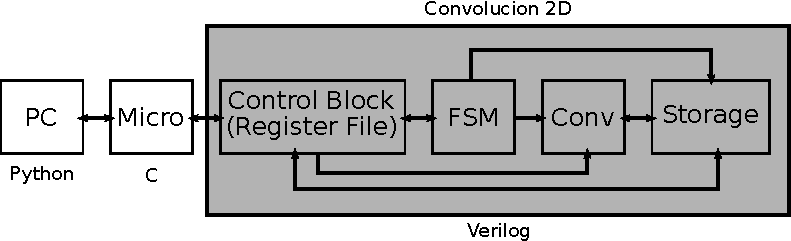
\includegraphics[width=3in]{workflow.pdf}
\caption{Flujo de trabajo del sistema y lenguajes en los que se trabaj\'o en
  cada instancia.}
\label{fig_workflow}
\end{figure}
La informaci\'on es entonces separada en lotes, el cliente env\'ia un
lote, espera a recibir el lote procesado y luego env\'ia el lote siguiente.

Un microprocesador instanciado en la FPGA es el encargado de recibir los lotes,
hace un desempaquetado de los datos y adem\'as le a\~nade a los mismos una 
cabecera necesaria para la comunicaci\'on con el m\'odulo de convoluci\'on.
Asimismo una vez que el m\'odulo finaliz\'o el procesamiento, el microprocesador 
toma esa informaci\'on procesada, la empaqueta y env\'ia nuevamente a la
computadora.

El m\'odulo de convoluci\'on procesa el lote, internamente es el Bloque de
Control (Control Block) quien hace de interfaz entre el resto del m\'odulo y el
exterior. La porci\'on de la imagen es almacenada, los bloques de convoluci\'on
(Conv) realizan la suma de los productos de los coeficientes del filtro con una
secci\'on de la imagen igual al tama\~no del filtro, una vez que toda la
porci\'on de la imagen fue procesada, se env\'ia el resultado y se espera a
recibir una nueva porci\'on. Una maquina de estados finita (FSM) lleva cuenta
del ciclo de entrada$\rightarrow$procesamiento$\rightarrow$salida que ocurre en
el m\'odulo.

\subsection{M\'odulo de convoluci\'on}
En esta secci\'on se describe en detalle la arquitectura del m\'odulo de
convoluci\'on.

\subsubsection{Almacenamiento de la informaci\'on}
El kernel o filtro que se quiere aplicar a la imagen se configura durante la
etapa de carga y es almacenado en registros de los bloques de convoluci\'on. Con
respecto a la imagen, se opt\'o por utilizar columnas de memoria, donde cada
columna almacena una columna de pixels. Queda entonces limitada la imagen a una
altura m\'axima dada por el n\'umero de direcciones accesibles en las columnas
de memoria.



\subsubsection{Estados}
Durante todo el ciclo de trabajo, el m\'odulo atraviesa distintos estados, en
primera instancia, est\'a en un estado inicial de \textbf{reset} esperando a ser
configurado

% An example of a floating figure using the graphicx package.
% Note that \label must occur AFTER (or within) \caption.
% For figures, \caption should occur after the \includegraphics.
% Note that IEEEtran v1.7 and later has special internal code that
% is designed to preserve the operation of \label within \caption
% even when the captionsoff option is in effect. However, because
% of issues like this, it may be the safest practice to put all your
% \label just after \caption rather than within \caption{}.
%
% Reminder: the "draftcls" or "draftclsnofoot", not "draft", class
% option should be used if it is desired that the figures are to be
% displayed while in draft mode.
%
%\begin{figure}[!t]
%\centering
%\includegraphics[width=2.5in]{myfigure}
% where an .eps filename suffix will be assumed under latex, 
% and a .pdf suffix will be assumed for pdflatex; or what has been declared
% via \DeclareGraphicsExtensions.
%\caption{Simulation results for the network.}
%\label{fig_sim}
%\end{figure}

% Note that the IEEE typically puts floats only at the top, even when this
% results in a large percentage of a column being occupied by floats.


% An example of a double column floating figure using two subfigures.
% (The subfig.sty package must be loaded for this to work.)
% The subfigure \label commands are set within each subfloat command,
% and the \label for the overall figure must come after \caption.
% \hfil is used as a separator to get equal spacing.
% Watch out that the combined width of all the subfigures on a 
% line do not exceed the text width or a line break will occur.
%
%\begin{figure*}[!t]
%\centering
%\subfloat[Case I]{\includegraphics[width=2.5in]{box}%
%\label{fig_first_case}}
%\hfil
%\subfloat[Case II]{\includegraphics[width=2.5in]{box}%
%\label{fig_second_case}}
%\caption{Simulation results for the network.}
%\label{fig_sim}
%\end{figure*}
%
% Note that often IEEE papers with subfigures do not employ subfigure
% captions (using the optional argument to \subfloat[]), but instead will
% reference/describe all of them (a), (b), etc., within the main caption.
% Be aware that for subfig.sty to generate the (a), (b), etc., subfigure
% labels, the optional argument to \subfloat must be present. If a
% subcaption is not desired, just leave its contents blank,
% e.g., \subfloat[].


% An example of a floating table. Note that, for IEEE style tables, the
% \caption command should come BEFORE the table and, given that table
% captions serve much like titles, are usually capitalized except for words
% such as a, an, and, as, at, but, by, for, in, nor, of, on, or, the, to
% and up, which are usually not capitalized unless they are the first or
% last word of the caption. Table text will default to \footnotesize as
% the IEEE normally uses this smaller font for tables.
% The \label must come after \caption as always.
%
%\begin{table}[!t]
%% increase table row spacing, adjust to taste
%\renewcommand{\arraystretch}{1.3}
% if using array.sty, it might be a good idea to tweak the value of
% \extrarowheight as needed to properly center the text within the cells
%\caption{An Example of a Table}
%\label{table_example}
%\centering
%% Some packages, such as MDW tools, offer better commands for making tables
%% than the plain LaTeX2e tabular which is used here.
%\begin{tabular}{|c||c|}
%\hline
%One & Two\\
%\hline
%Three & Four\\
%\hline
%\end{tabular}
%\end{table}


% Note that the IEEE does not put floats in the very first column
% - or typically anywhere on the first page for that matter. Also,
% in-text middle ("here") positioning is typically not used, but it
% is allowed and encouraged for Computer Society conferences (but
% not Computer Society journals). Most IEEE journals/conferences use
% top floats exclusively. 
% Note that, LaTeX2e, unlike IEEE journals/conferences, places
% footnotes above bottom floats. This can be corrected via the
% \fnbelowfloat command of the stfloats package.




\section{Conclusion}
The conclusion goes here.




% conference papers do not normally have an appendix



% use section* for acknowledgment
\ifCLASSOPTIONcompsoc
  % The Computer Society usually uses the plural form
  \section*{Acknowledgments}
\else
  % regular IEEE prefers the singular form
  \section*{Acknowledgment}
\fi


The authors would like to thank...





% trigger a \newpage just before the given reference
% number - used to balance the columns on the last page
% adjust value as needed - may need to be readjusted if
% the document is modified later
%\IEEEtriggeratref{8}
% The "triggered" command can be changed if desired:
%\IEEEtriggercmd{\enlargethispage{-5in}}

% references section

% can use a bibliography generated by BibTeX as a .bbl file
% BibTeX documentation can be easily obtained at:
% http://mirror.ctan.org/biblio/bibtex/contrib/doc/
% The IEEEtran BibTeX style support page is at:
% http://www.michaelshell.org/tex/ieeetran/bibtex/
%\bibliographystyle{IEEEtran}
% argument is your BibTeX string definitions and bibliography database(s)
%\bibliography{IEEEabrv,../bib/paper}
%
% <OR> manually copy in the resultant .bbl file
% set second argument of \begin to the number of references
% (used to reserve space for the reference number labels box)
\bibliographystyle{IEEEtran}
\bibliography{PROJECT_DOC}
%\begin{thebibliography}{1}
%
%\bibitem{IEEEhowto:kopka}
%H.~Kopka and P.~W. Daly, \emph{A Guide to \LaTeX}, 3rd~ed.\hskip 1em plus
  %0.5em minus 0.4em\relax Harlow, England: Addison-Wesley, 1999.
%
%\end{thebibliography}




% that's all folks
\end{document}


